\documentclass{article}


\usepackage{amsmath}
\usepackage{amssymb}
\usepackage{cancel}
\usepackage{graphicx}
\usepackage{float}
\usepackage{matlab-prettifier}
\usepackage[margin=1.0in]{geometry}




% bold letters
\newcommand{\bola}{\mathbf{a}}
\newcommand{\bolc}{\mathbf{c}}
\newcommand{\bolf}{\mathbf{f}}
\newcommand{\bolg}{\mathbf{g}}
\newcommand{\boll}{\mathbf{l}}
\newcommand{\bolq}{\mathbf{q}}
\newcommand{\bolp}{\mathbf{p}}
\newcommand{\bolu}{\mathbf{u}}
\newcommand{\bolv}{\mathbf{v}}
\newcommand{\bolw}{\mathbf{w}}
\newcommand{\bolz}{\mathbf{z}}

\newcommand{\bolA}{\mathbf{A}}
\newcommand{\bolB}{\mathbf{B}}
\newcommand{\bolC}{\mathbf{C}}
\newcommand{\bolD}{\mathbf{D}}
\newcommand{\bolE}{\mathbf{E}}
\newcommand{\bolF}{\mathbf{F}}
\newcommand{\bolG}{\mathbf{G}}
\newcommand{\bolH}{\mathbf{H}}
\newcommand{\bolI}{\mathbf{I}}
\newcommand{\bolJ}{\mathbf{J}}
\newcommand{\bolK}{\mathbf{K}}
\newcommand{\bolL}{\mathbf{L}}
\newcommand{\bolM}{\mathbf{M}}
\newcommand{\bolN}{\mathbf{N}}
\newcommand{\bolO}{\mathbf{O}}
\newcommand{\bolP}{\mathbf{P}}
\newcommand{\bolQ}{\mathbf{Q}}
\newcommand{\bolR}{\mathbf{R}}
\newcommand{\bolS}{\mathbf{S}}
\newcommand{\bolT}{\mathbf{T}}
\newcommand{\bolU}{\mathbf{U}}
\newcommand{\bolV}{\mathbf{V}}
\newcommand{\bolW}{\mathbf{W}}
\newcommand{\bolX}{\mathbf{X}}
\newcommand{\bolY}{\mathbf{Y}}
\newcommand{\bolZ}{\mathbf{Z}}

% bold symbols
\newcommand{\bolalpha}{\boldsymbol{\alpha}}
\newcommand{\bolbeta}{\boldsymbol{\beta}}
\newcommand{\boleta}{\boldsymbol{\eta}}
\newcommand{\bolpsi}{\boldsymbol{\psi}}

% shadowed letters
\newcommand{\PP}{\mathbb{P}}
\newcommand{\RR}{\mathbb{R}}
\newcommand{\CC}{\mathbb{C}}
\newcommand{\ZZ}{\mathbb{Z}}

% mathcal letters
\newcommand{\calA}{\mathcal{A}}
\newcommand{\calB}{\mathcal{B}}
\newcommand{\calC}{\mathcal{C}}
\newcommand{\calD}{\mathcal{D}}
\newcommand{\calE}{\mathcal{E}}
\newcommand{\calF}{\mathcal{F}}
\newcommand{\calG}{\mathcal{G}}
\newcommand{\calH}{\mathcal{H}}
\newcommand{\calI}{\mathcal{I}}
\newcommand{\calJ}{\mathcal{J}}
\newcommand{\calK}{\mathcal{K}}
\newcommand{\calL}{\mathcal{L}}
\newcommand{\calM}{\mathcal{M}}
\newcommand{\calN}{\mathcal{N}}
\newcommand{\calO}{\mathcal{O}}
\newcommand{\calP}{\mathcal{P}}
\newcommand{\calQ}{\mathcal{Q}}
\newcommand{\calR}{\mathcal{R}}
\newcommand{\calS}{\mathcal{S}}
\newcommand{\calT}{\mathcal{T}}
\newcommand{\calU}{\mathcal{U}}
\newcommand{\calV}{\mathcal{V}}
\newcommand{\calW}{\mathcal{W}}
\newcommand{\calX}{\mathcal{X}}
\newcommand{\calY}{\mathcal{Y}}
\newcommand{\calZ}{\mathcal{Z}}


% derivatives
\newcommand{\pp}[2]{\frac{\partial #1}{\partial #2}}
\newcommand{\dd}[2]{\frac{d #1}{d #2}}


% fraction shortcut
\newcommand{\f}[2]{\frac{#1}{#2}}
\newcommand{\slfrac}[2]{\left.#1\middle/#2\right.}

% common operators
\newcommand{\vvvert}{|\kern-1pt|\kern-1pt|}
\newcommand{\enorm}[1]{\vvvert #1 \vvvert}


% matrices
\newcommand{\bmat}[1]{\left(\begin{array}{#1}}
\newcommand{\emat}{\end{array}\right)} 



\newcommand{\blist}{\begin{list}{\ballrefb}{\leftmargin=2.0em}
  \setlength{\itemsep}{2pt}
  \setlength{\parskip}{0pt}}
\newcommand{\elist}{\end{list}}



% common format strings
\def\etal{{\it et al.}}
\def\ie{{\it i.e.}}
\def\eg{{\it e.g.}}


\DeclareMathOperator*{\arginf}{arg\,inf}
\DeclareMathOperator*{\argsup}{arg\,sup}
\DeclareMathOperator*{\argmax}{arg\,max}
\DeclareMathOperator*{\argmin}{arg\,min}


\begin{document}
\Large\centering AER1418: Assignment 3\\
\normalsize\raggedright Geoff Donoghue \hfill April 1, 2019\\

\section*{Part 1. Heat equation with discontinuous conductivity}
We consider a one-dimensional heat equation over the unit domain \(\Omega \equiv (0,1) \), in the trial space \(\calV \equiv \{v \in H^1(\Omega) | v(x=0) = 0 \} \) we seek some solution \(u \in \calV \) such that
\begin{equation*}
	\int_0^1 \kappa(x) \dd{v}{x}\dd{u}{x}dx = v(x=1) \quad \forall v \in \calV,
\end{equation*}
where we have a discontinuous heat conductivity given by
\begin{equation*}
	\kappa(x) = 
	\begin{cases}
	1\quad x \in (0,1/2)\\
	2\quad x \in (1/2,1).
	\end{cases}
\end{equation*}
\begin{itemize}
	\item[(a)] In order to analytically compute the weak solution to this heat conduction problem we will first split the domain in half and integrate by parts to obtain
	\begin{equation*}
		-\int_0^\frac{1}{2}v\dfrac{d^2u}{dx^2}dx + \left.2v\dd{u}{x}\right|_{x=1} - \left.v\dd{u}{x}\right|_{x=1/2} - 2\int_\frac{1}{2}^1v\dfrac{d^2u}{dx^2}dx = v(x=1).
	\end{equation*}
	If we hope to enforce the above equation in a point-wise sense we must satisfy the following equations
	\begin{equation*}
		\kappa(x)\dfrac{d^2u}{dx^2} = 0 \quad x \in (0,1),\quad \left.\dd{u}{x}\right|_{x=1} = \dfrac{1}{2},\quad \left.\dd{u}{x}\right|_{x=\frac{1}{2}} = 0,\quad u(x=0)=0,
	\end{equation*}
	where the last equation is a Dirichlet boundary condition enforced by the trial space in the weak form of the problem. Immediately we see that the solution will take the form of a piecewise linear polynomial, by applying the conditions at the left and right boundaries we obtain
	\begin{equation*}
		u = \begin{cases} c_Lx \quad\quad x\in(0,1/2)\\ \frac{1}{2}x + c_R\quad x\in(1/2,1).
		\end{cases}
	\end{equation*}
	To enforce our interface condition (and also to ensure our solution is \(\in \calV\)) we will say that 
	\begin{equation*}
		\left.\dd{u}{x}\right|_{x=\frac{1}{2}} = 0 \implies \lim\limits_{\epsilon\to0}u(\frac{1}{2} + \epsilon) = \lim\limits_{\epsilon\to0} u(\frac{1}{2} - \epsilon).
	\end{equation*}
	Applying this condition yields \(c_R = \dfrac{2c_L-1}{4} \). We can say that 
	\begin{equation*}
		\int_0^1\kappa(x)\dd{v}{x}\dd{u}{x}dx = 1\int_0^\frac{1}{2}c_L\dd{v}{x}dx + 2\int_\frac{1}{2}^1\frac{1}{2}\dd{v}{x}dx = c_Lv(\frac{1}{2}) + v(1) - v(\frac{1}{2}),
	\end{equation*}
	and note that \(c_L = 1 \) will satisfy the weak problem \(\forall v \in \calV \). The solution is therefore given by
	\begin{equation*}
		u = \begin{cases} \quad x \quad\quad x\in(0,1/2)\\ \frac{1}{2}x + \frac{1}{4}\quad x\in(1/2,1).
		\end{cases}
	\end{equation*}
	Furthermore, since we have a coercive and continuous bilinear form and a continuous linear form, by the Lax-Milgram theorem this solution is unique. For completeness we can verify that our solution is \(\in \calV \). The only nontrivial part of this involves proving the existence and boundedness of the weak derivative of \(u\). It can be shown that the first weak derivative exists, but the second does not so the solution is \(\in H^1(\Omega) \), but \(\notin H^2{\Omega} \).%To do so we find, 
%	\begin{align*}
%		\int_{0}^{1}v\dd{u}{x}dx = 
%	\end{align*}
	
	\item[(b)] Since we have \(\Omega \subset \RR \) as a Lipschitz domain, \(H^1_0(\Omega) \subset \calV \subset H^1(\Omega) \), our bilinear form is coercive and continuous, our linear form is continuous, and \(\calV_h \equiv \{v\in V | v \in \PP^1(K), K \in \calT_h^\text{even} \} \subset \calV \) we can use C\'ea's lemma 
	\begin{equation*}
		\|u - u_h\|_\calV \leq \dfrac{\gamma}{\alpha}\inf\limits_{w_h \in \calV_h}\|u - w_h\|_\calV.
	\end{equation*}
	Where \(\gamma \) and \(\alpha \) are the continuity and coercivity constants for the bilinear form, respectively. We note that \(\|\cdot\|_\calV = \|\cdot\|_{H^1(\Omega)} \), and that since our analytical solution \(u\) can be expressed as an element of our approximation space (i.e. \(u \in \calV_h \)), we can therefore say that 
	\begin{equation*}
		\inf\limits_{w_h \in \calV_h}\|u - w_h\|_\calV = 0.
	\end{equation*}
	Where evaluating the integral to determine the infinimum is very straightforward, and is therefore omitted. As a result of the infinimum of the error being zero in our approximation space, we say that \(\|u-u_h\|_{H^1(\Omega)} = 0\).
	
	\item[(c)] We now update our approximation space to consist of quadratic piecewise polynomials, and note that \(\calV'_h \equiv \{v\in \calV | v \in \PP^2(K), K \in \calT_h^\text{even} \} \supset \calV_h \). Since any approximation in \(\calV_h \) exists in \(\calV'_h \) the infinimum is again zero; furthermore, the conditions required to invoke C\'ea's lemma are again satisfied, and we can again state that \(\|u-u_h\|_{H^1(\Omega)} = 0\).
	
	\item[(d)] We no longer have \(u \in \calV_h \), we note that on every element except for the one located in the middle of the domain (\(K_\text{mid} \)) the solution can be approximated exactly and therefore note that
	\begin{equation*}
		\|u-u_h\|_{H^1(\Omega)} = \|u-u_h\|_{H^1(K_\text{mid})} \geq |u-u_h|_{H^1(K_\text{mid})} \geq \inf\limits_{w_h\in\calV_h}|u-w_h|_{H^1(K_\text{mid})}.
	\end{equation*}
	We can deduce the derivative of the best-fit solution to be \(\dd{w_h}{x} = \frac{3}{4}\) and state that
	\begin{align*}
	\inf\limits_{w_h\in \calV_h}|u-w_h|_{H^1(K_\text{mid})} =& \inf\limits_{w_h\in \calV_h}\left(\int_{K_\text{mid}}\left(\dd{u}{x} - \dd{w_h}{x} \right)^2dx \right)^{1/2}\\
	=& \left[\int_{\frac{1-h}{2}}^\frac{1}{2}(1-\dfrac{3}{4})^2dx + \int_{\frac{1}{2}}^\frac{1+h}{2}(\dfrac{1}{2} - \dfrac{3}{4})^2dx\right]^{1/2}\\
	=& \left[\left.\dfrac{x}{16} \right|_{\frac{1-h}{2}}^\frac{1}{2} + \left.\dfrac{x}{16} \right|_\frac{1}{2}^\frac{1+h}{2} \right]^{1/2}\\
	=& \dfrac{1}{4}h^{1/2}.
	\end{align*}
	We can therefore state that the smallest \(r\) such that 
	\begin{equation*}
		\|u - u_h\|_{H^1(\Omega)} \geq Ch^r = \dfrac{1}{4}h^{1/2}
	\end{equation*}
	is \(r = 1/2\).
	
	\item[(e)] Similarly to the previous problem, we now deduce the derivative of the best-fit solution to be \(\dd{w_h}{x} = mx+b \), with \(m = -\frac{1}{2h} \), and \(b = \frac{3h+1}{4h}\). We can substitute this into our infinimum expression to obtain
	\begin{align*}
		\inf\limits_{w_h\in \calV_h}|u-w_h|_{H^1(K_\text{mid})} =& \inf\limits_{w_h\in \calV_h}\left(\int_{K_\text{mid}}\left(\dd{u}{x} - \dd{w_h}{x} \right)^2dx \right)^{1/2} \\
		=& \left[\int_{\frac{1-h}{2}}^\frac{1}{2}(1+\dfrac{x}{2h}-\dfrac{3h+1}{4h})^2dx + \int_{\frac{1}{2}}^\frac{1+h}{2}(\dfrac{1}{2}+\dfrac{x}{2h}-\dfrac{3h+1}{4h})^2dx\right]^{1/2}\\
		=& \left[\dfrac{h}{96} + \dfrac{h}{96} \right]^{1/2}\\
		=& \dfrac{1}{\sqrt{48}}h^{1/2}
	\end{align*}
	Where I have evaluated the integral using wolfram alpha. We see that our value for \(r\) is once again \(\dfrac{1}{2} \). This goes to show that since our solution is not sufficiently regular in \(H^{s+1}(\calT_h) \). We expect \(r \equiv \min\{s,p\} \), and can deduce that \(s = \frac{1}{2}\).
\end{itemize}

\section*{Part 2. Verification: method of manufactured solution}
\begin{itemize}
	\item[(a)] For the \(\PP^1 \) and \(\PP^2 \) finite element approximations we expect that if our solution is smooth our \(H^1(\Omega) \) error norm will converge at a rate of \(p\). A convergence plot of the error against \(h\) is shown in Figue \ref{fig:mms_h1} below.
	\begin{figure}[H]
		\centering
		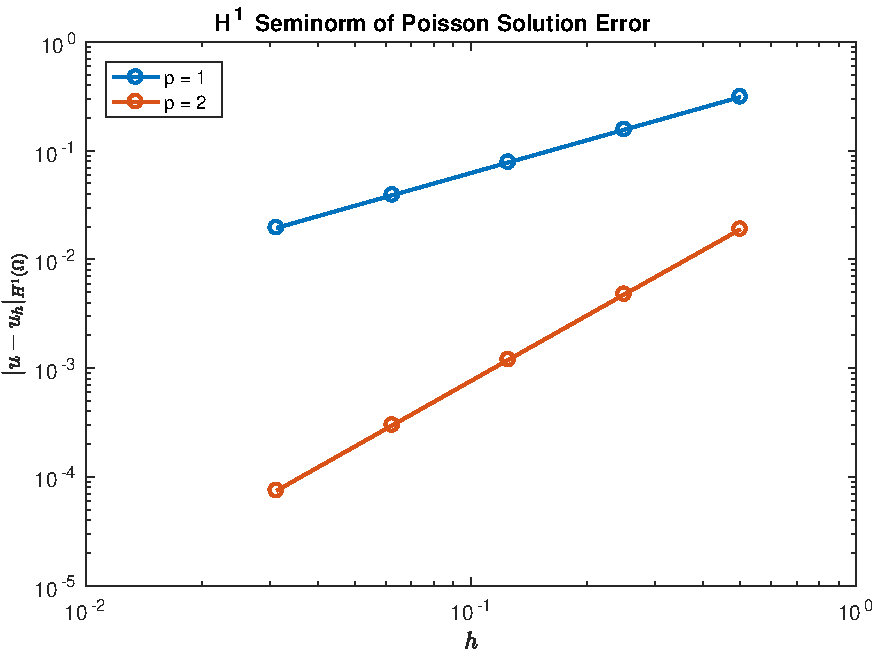
\includegraphics[width=0.6\textwidth]{MMS_H1_conv.pdf}
		\caption{\(H^1(\Omega)\) semi norm error convergence for Poisson 1D MMS problem.}
		\label{fig:mms_h1}
	\end{figure}
	The convergence rates were found to be \(1.0000\) and \(1.9998\) for the \(\PP^1 \) and \(\PP^2 \) approximations, respectively; these rates agree very well with the theory.
	\item[(b)] For the \(\PP^1 \) and \(\PP^2 \) finite element approximations we expect that if our solution is smooth our \(H^1(\Omega) \) error norm will converge at a rate of \(p+1\). A convergence plot of the error against \(h\) is shown in Figure \ref{fig:mms_l2} below.
	\begin{figure}[H]
		\centering
		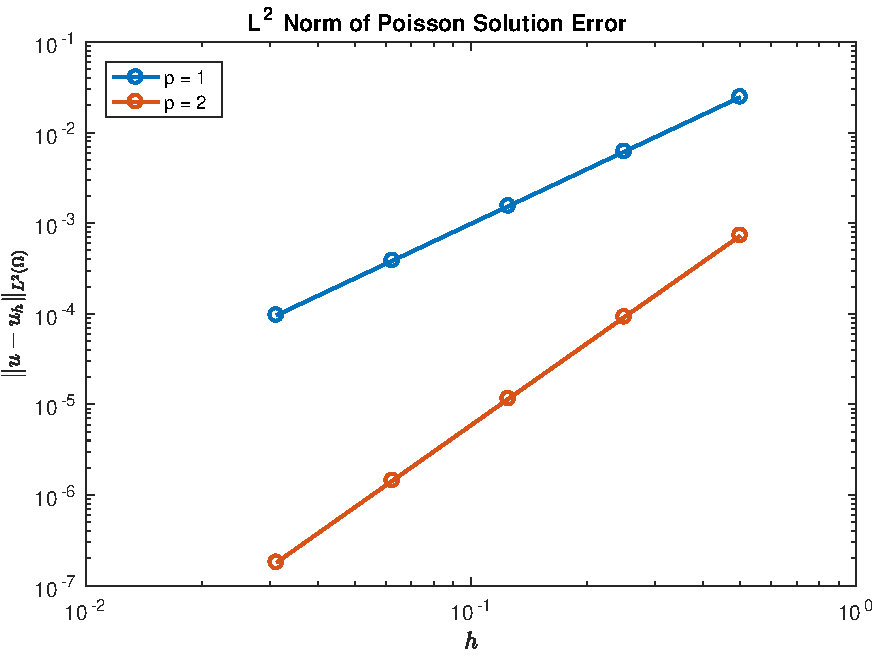
\includegraphics[width=0.6\textwidth]{MMS_L2_conv.pdf}
		\caption{\(L^2(\Omega)\) norm error convergence for Poisson 1D MMS problem.}
		\label{fig:mms_l2}
	\end{figure}
	The convergence rates were found to be \(2.0000\) and \(2.9998\) for the \(\PP^1 \) and \(\PP^2 \) approximations, respectively; these rates agree very well with the theory.
	\item[(c)] For the \(\PP^1 \) and \(\PP^2 \) finite element approximations we may na\"ively expect that if our solution is smooth our output error \(|\ell^\text{o}(u) - \ell^\text{o}(u_h)| \) will converge at a rate of \(2p\). We can however note that since our problem satisfies assumptions 6.1, 6.2, and 6.3 from the notes, and our primal and adjoint solutions are \(\in H^1(\Omega) \cap H^{s(')+1}(\calT_h) \) we have
	\begin{equation*}
		|\ell^\text{o}(u) - \ell^\text{o}(u_h)| \lesssim h^{r+r'}|u|_{H^{r+1}(\calT_h)}|\psi|_{H^{r'+1}(\calT_h)}
	\end{equation*}
	with \(r \equiv \min\{s,p\} \) and \(r' \equiv \min\{s',p\} \). Our adjoint equation is given by: find \(\psi \in \calV \) such that 
	\begin{equation*}
		a(w,\psi) = \ell^\text{o}(w) \quad \forall w \in \calV.
	\end{equation*}
	We will solve this equation by first converting from the weak form to its strong form by integrating by parts, the weak form of the adjoint problem is
	\begin{equation*}
		w(x=1)\left.\dd{\psi}{x}\right|_{x=1} - \cancel{w(x=0)}\left.\dd{\psi}{x}\right|_{x=0} = \int_\Omega w (1+\dfrac{d^2\psi}{dx^2})dx.
	\end{equation*}
	We can deduce form here that the strong form of the problem is 
	\begin{equation*}
		-\dfrac{d^2\psi}{dx^2} = 1, \quad \psi(x=0) = 0, \quad \left.\dd{\psi}{x}\right|_{x=1} = 0,
	\end{equation*}
	the solution of which is
	\begin{equation*}
		\psi = x - \dfrac{x^2}{2},
	\end{equation*}
	i.e. a second order polynomial, for which \(|\psi|_{H^{r'+1}(\calT_h)} = 0 \), where \(r' = p \).
	
	A convergence plot of the error against \(h\) is shown in Figue \ref{fig:mms_out} below.
	\begin{figure}[H]
		\centering
		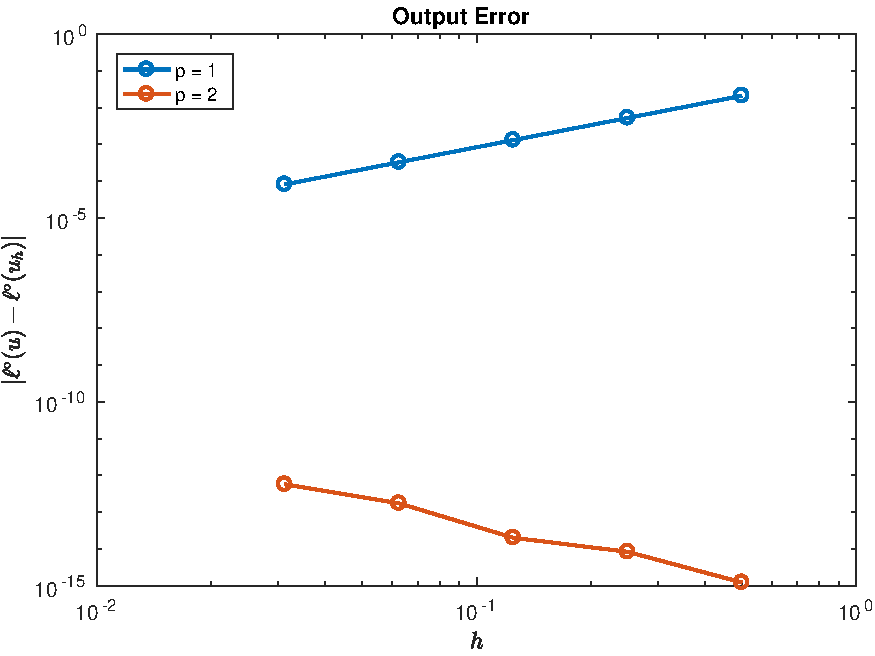
\includegraphics[width=0.6\textwidth]{MMS_output_conv.pdf}
		\caption{Output error convergence for Poisson 1D MMS problem.}
		\label{fig:mms_out}
	\end{figure}
	The convergence rates were found to be \(2.0001\) and \(-1.7175\) for the \(\PP^1 \) and \(\PP^2 \) approximations, respectively. The second convergence rate is expected to be zero in the absence of quadrature error (we use \(p_{quad} = 4p\)), which will be proportional to the number of elements. 
\end{itemize}

\section*{Part 3. Linear Elasticity}
We can describe our problem with the following equations
\begin{equation*}
	-\nabla \cdot \sigma(u) = 0 \text{ in } \Omega, \quad u = u^B \text{ on } \Gamma_D, n\cdot \sigma(u) = g \text{ on } \Gamma_N.
\end{equation*}
We have \(\Omega \equiv (0,2)\times(0,1/2) \), \(\Gamma_N \equiv \Gamma_\text{right} = \{2\}\times(0,1/2) \), \(\Gamma_D = \partial\Omega/\Gamma_\text{right} \), and \(g = \left[g_{\text{pull}}\; 0\right]^T \). Multiplying by a test function and integrating by parts yields the weak form of our problem
\begin{equation*}
	\int_{\Omega} \nabla v : \sigma(u)dx = \int_{\Gamma_\text{right}}v\cdot gds
\end{equation*}
By substituting in our expression for stress in terms of strain and noting that because \(\epsilon(u)\) is symmetric, we have \(\nabla v : \epsilon(u) = \epsilon(v):\epsilon(u) \) we can rewrite our weak form as
\begin{equation*}
	\int_{\Omega} 2 \mu \epsilon(v):\epsilon(u) + \lambda\text{tr}(\epsilon(v))(\epsilon(u))dx = \int_{\Gamma_\text{right}}v\cdot gds.
\end{equation*}
Here we will define our bilinear and linear forms to be respectively
\begin{equation*}
	a(w,v) \equiv\int_{\Omega} 2 \mu \epsilon(v):\epsilon(w) + \lambda\text{tr}(\epsilon(v))(\epsilon(w))dx , \quad \ell(v) \equiv  \int_{\Gamma_\text{right}}v\cdot gds.
\end{equation*}
\begin{itemize}
	\item[(a)] Twice the strain energy density integrated over the domain is
	\begin{alignat*}
		2\int_{\Omega}W(u)dx =& 2\int_\Omega \dfrac{1}{2}\epsilon(u):\sigma(u)dx &&(\text{Def. of } W(u))\\
		=& \int_{\Omega} \epsilon(u) : \left[2 \mu \epsilon(u) + \lambda\text{tr}(\epsilon(u))I\right] dx &&(\text{Def. of } \sigma(u))\\
		=& \int_{\Omega} 2 \mu \epsilon(u):\epsilon(u) + \lambda\text{tr}(\epsilon(u))(\epsilon(u))dx \\
		=& a(u,u) &&(\text{Def. of } a(u,u))\\
		=& \ell(u) &&(\text{Def. of } u)\\
		=& \int_{\Gamma_\text{right}}u\cdot gds &&(\text{Def. of } \ell(u))\\
		=& \int_{\Gamma_\text{right}}u_1 g_{\text{pull}}ds &&(\text{Def. of } g(u))\\
		=& \ell^\text{o}(u) &&(\text{Def. of } \ell^\text{o}(u)),
	\end{alignat*}
	which is exactly our compliance ouput. 
	
	\item[(b)] Our problem satisfies all the requirements for a minimization formulation with an energy functional 
	\begin{equation*}
		u = \argmin\limits_{w\in\calV} J(w), \quad J(v) \equiv \dfrac{1}{2}a(v,v) - \ell(v) \quad \forall v \in \calV.
	\end{equation*}
	Likewise we have a finite elemenet approximation of the above
	\begin{equation*}
		u_h = \argmin\limits_{w_h\in\calV_h} J(w_h), \quad J(v) \equiv \dfrac{1}{2}a(v,v) - \ell(v) \quad \forall v \in \calV_h.
	\end{equation*}
	We note that since \(\calV_h \subset \calV \) we can say that
	\begin{equation*}
		J(u) \leq J(u_h), \implies \dfrac{1}{2}a(u,u) - \ell(u) \leq \dfrac{1}{2}a(u_h,u_h) - \ell(u_h).
	\end{equation*}
	The definitions of \(u\) and \(u_h\) imply that \(a(u,u) = \ell(u) \) and  \(a(u_h,u_h) = \ell(u_h) \), therefore
	\begin{equation*}
		\dfrac{1}{2}\ell(u) - \ell(u) \leq \dfrac{1}{2}\ell(u_h) - \ell(u_h).
	\end{equation*}
	Since we have \(\ell(u) = \ell^\text{o}(u) \) and \(\ell(u_h) = \ell^\text{o}(u_h) \) we can say
	\begin{equation*}
		-\dfrac{1}{2}\ell^\text{o}(u) \leq -\dfrac{1}{2}\ell^\text{o}(u_h).
	\end{equation*}
	This implies that 
	\begin{equation*}
		\ell^\text{o}(u_h) \leq \ell^\text{o}(u).
	\end{equation*}
	\item[(c)] The code used to solve this problem is shown:
	\lstinputlisting[style=Matlab-editor, linerange={1-212}]{../fem2d_part/driver/plate.m}
	\item[(d)] Figure \ref{refsoln} shows the solution for which the reference output is calculated. It uses 28649 elements (\(h = 0.008 \)) and yields a compliance output of \(\ell^\text{o}(u_\text{ref}) = 0.00456145212 \)
	\begin{figure}[H]
		\centering
		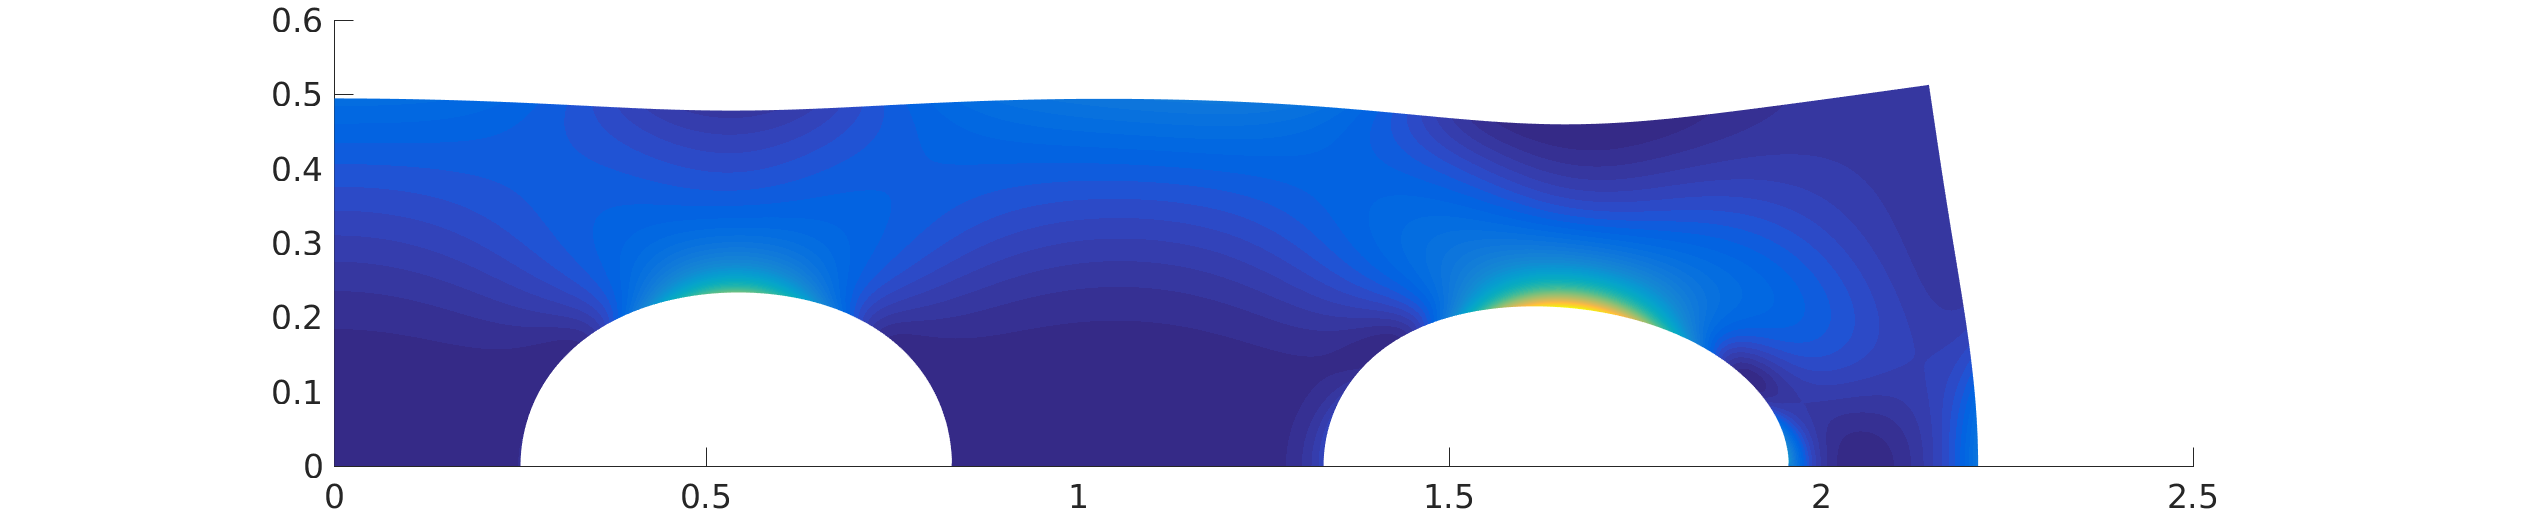
\includegraphics[width=0.95\textwidth]{test.pdf}
		\caption{Strain energy density field on the deformed mesh.}
		\label{refsoln}
	\end{figure}
	\item[(e)] Reference outputs for each family of approximations are summarized in Table \ref{table1}
			   
			   \begin{table}[H]
			   	\centering
			   	\begin{tabular}{r||c|c|c}
			   		& A1 & A2 & A3 \\
			   		\hline
			   		\(\ell^\text{o}(u_h)\) & 0.0045588902 & 0.0045610541 & 0.0045614521\\
			   	\end{tabular}
			   	\caption{Reference compliance outputs, for each approximation family}
			   	\label{table1}
			   \end{table}
	\item[(f)] Figure \ref{out_conv} shows a semilog plot of \(\ell^\text{o}(u_h) \) against the number of degrees of freedom for each of our approximation families; the reference output is also shown. From part (b) we expect that \(\ell^\text{o}(u_h) < \ell^\text{o}(u_\text{ref})\) for each solution. 
	\begin{figure}[H]
		\centering
		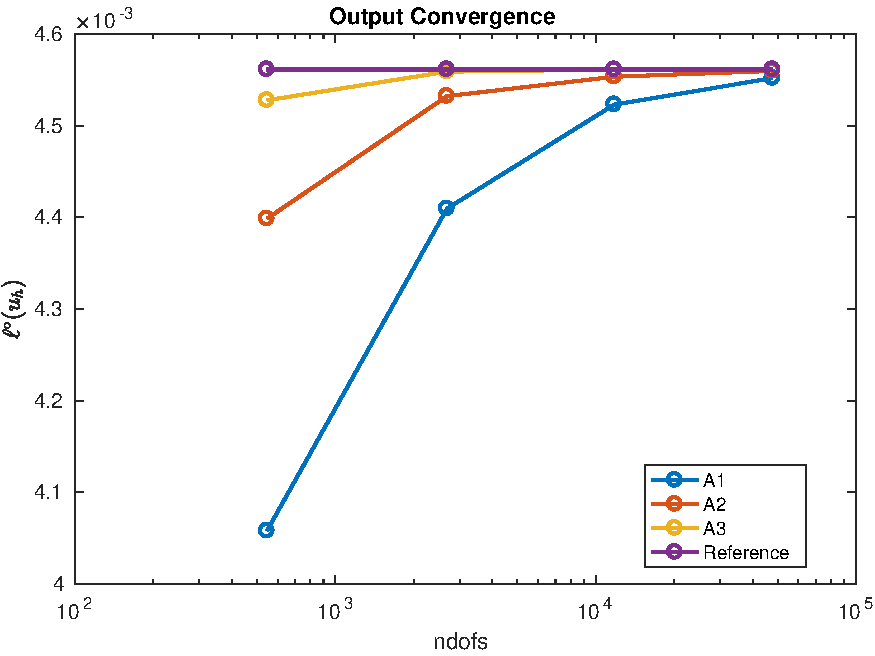
\includegraphics[width=0.6\textwidth]{Plate_output_conv.pdf}
		\caption{Compliance output for several approximations, note the monotonicity.}
		\label{out_conv}
	\end{figure}
	We note that as expected, \(\ell^\text{o}(u_h) < \ell^\text{o}(u_\text{ref})\), for each solution. 
	\item[(g)] A plot showing a log-log relation between \(|\ell^\text{o}(u_h) - \ell^\text{o}(u_\text{ref})| \) against the number of degrees of freedom for each approximation family is shown in Figure \ref{out_err_conv} below. 
	\begin{figure}[H]
		\centering
		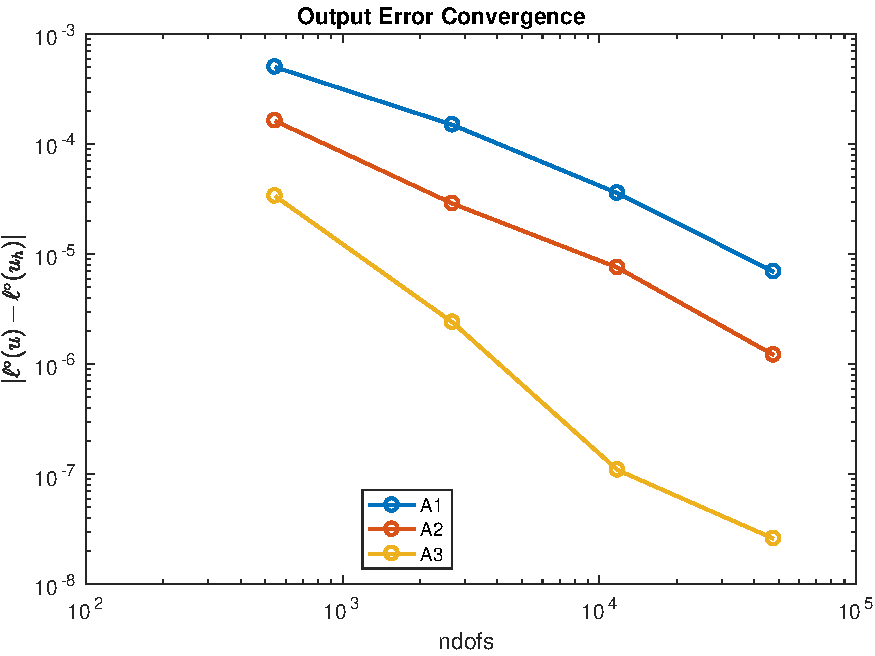
\includegraphics[width=0.6\textwidth]{Plate_output_error_conv.pdf}
		\caption{Compliance output error convergence.}
		\label{out_err_conv}
	\end{figure}
	\item[(h)] The slopes of the above plot are:\\
		\begin{table}[H]
			\centering
			\begin{tabular}{r||c|c|c}
				& A1 & A2 & A3 \\
				\hline
				m & -0.8596 & -1.0001 & -1.8673\\
			\end{tabular}
			\caption{Compliance output error convergence rates with respect to ndofs}
			\label{table2}
		\end{table}
		We may also compute the convergence rates with respect to \(h\), these are:\\
		\begin{table}[H]
			\centering
			\begin{tabular}{r||c|c|c}
				& A1 & A2 & A3 \\
				\hline
				r & 1.9042 & 2.2153 & 4.1364\\
			\end{tabular}
			\caption{Compliance output error convergence rates with respect to \(h\)}
			\label{table3}
		\end{table}
		
		Which are approximately twice the negative convergence rates with respect to the number of degrees of freedom, this is expected as ndofs \(\sim 1/h^2 \).
		
		Furthermore, we note that if \(u \in H^1(\Omega) \cap H^{s+1}(\calT_h) \) and \(\psi \in H^1(\Omega) \cap H^{s'+1}(\calT_h) \) then we have
		\begin{equation*}
			|\ell^\text{o}(u_h) - \ell^\text{o}(u_\text{ref})| \lesssim h^{r+r'}|u|_{H^{r+1}(\calT_h)}|\psi|_{H^{r'+1}(\calT_h)},
		\end{equation*}
		where \(r \equiv \min\{s,p\}, r' \equiv \min\{s',p\} \). Since we can achieve \(r=2p\) convergence we can conclude that \(s > 2\) or that \(u \in H^{k\geq3}(\Omega) \).
		
\end{itemize}

\section*{Appendix}
	Here is additional code, used in part 2; code used to generate refinement plots is simple and therefore not included.
	\lstinputlisting[style=Matlab-editor, linerange={125-202}]{../fem2d_part/driver/poisson1d.m}
\end{document}